\section{Graph Query Languages limitations’ on Graph Nesting}
\subsection{Graph Joins' limitations in providing the $\nu_\cong$ operator}\label{sec:whynotjoins}
\begin{figure}[!b]

\end{figure}

\begin{figure*}
	\begin{minipage}{\textwidth}
\centering
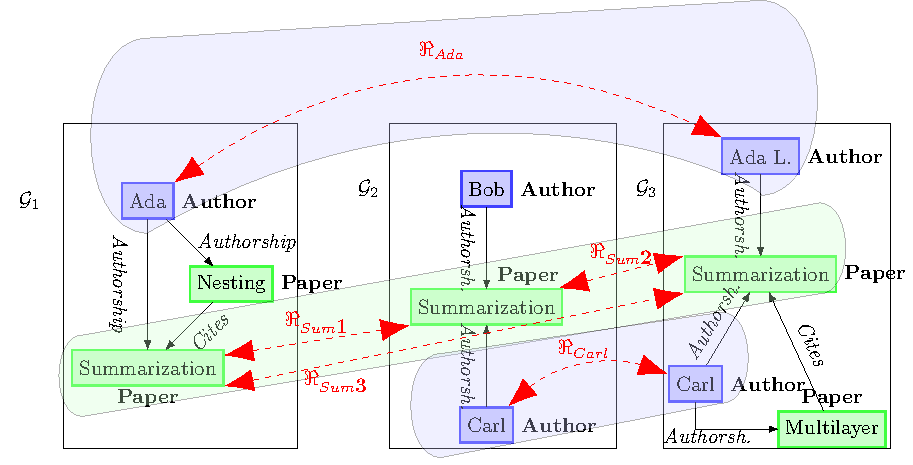
\includegraphics[width=\textwidth]{fig/06nesting/01_example}
\subcaption{Cleaned sources resulting from the
	transformation phase. The shaded areas represent distinct 
	graphs indicating which vertices (Authors and Papers) must be considered as the same entity.}
\label{fig:homog}
	\end{minipage}
	\begin{minipage}{\textwidth}

\centering
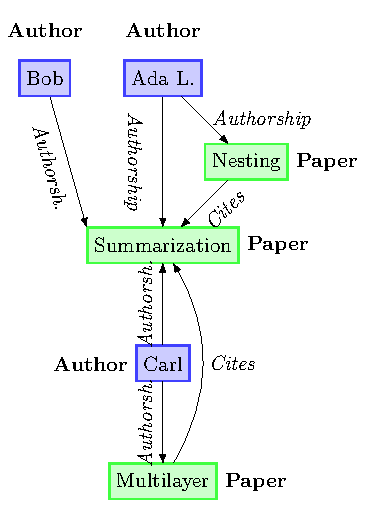
\includegraphics[scale=1]{fig/06nesting/02_result}
\subcaption{Representing the expected output $G_{out}$ for the data integration phase, ready to be fit to the graph datawarehouse.}
\label{fig:expresult}
\end{minipage}
\caption{$\nu_\cong$: another use case requiring the nesting operator $\nu$, as required by the last step of the data integration process before actually performing the queries over the integrated data. This last chapter ends the thesis by providing an example of the last operator required for such data integration process. In this case the outcome of the clustering operator is a similarity predicate $\cong$ using a entity-resolution process.}
\end{figure*}
We now discuss a use case where the graph nesting approach aggregates similar nodes into one single representation while discarding the original sources' pieces of information. Please refer to Section \vref{subsec:queryrw} for the general data integration scenario where such operator ($\nu_\cong$, that is grouping over an equivalence classifier $\cong$) may be adopted. In particular, we are going to show that, even though full graph join may represent this procedure, the resulting solution may be hardly implementable. To make our point, we are going to provide a different use case from the one previously offered.

\begin{example}
    Suppose to integrate, within a graph ETL, three distinct bibliographic sources (e.g. DBLP, Microsoft Academic Graph, Google Scholar) into one final graph. Each of these separately undergoes a data cleaning phase and are represented as the distinct connected components after an entity resolution processes \cite{markus}. Such components are represented by the graphs $G_1$, $G_2$ and $G_3$ in Figure \ref{fig:homog}.
As a next step, the entity resolution \cite{ALIEH17} analyses if nodes are appearing in the different sources and representing the same entity: as a consequence, we create the red relations in Figure \ref{fig:homog}, and then collect them into graphs representing a clique of all the resolved entities. The outcome of this operation is provided in Figure \vref{fig:expresult}, where all the entities representing one single entity are merged into one single vertex.
\end{example}

Another example where such edge joins could be of some use is within the ontology alignment process provided in Definition \vref{def:ontolalignment}. For instance, we can interpret each description logic axiom $C\sqsubseteq C'$ as an oriented edge connecting each vertex of the graph satisfying the predicate $C$ to the ones satisfying $C'$, thus allowing to join two graphs which schemas were previously aligned.

    The class of graph $\otimes_\theta$ products could be then generalised to support edges $E$ as a basis for the definition of the $\theta$ predicates. In particular, such predicate $\theta_E$ can be defined over a set of edges $E$ as follows:
	\[\theta_E(a,b)\Leftrightarrow \exists e\in E. \lambda(e)=(a,b)\]
	In such cases, we will write the predicate $\theta_E$ directly as $E$ through abuse of notation allowing to list the edges involved within the join operation directly. We can now ask ourselves if the following expression provides $G_{out}$ in Figure \ref{fig:expresult}:
\[(G_1\fullouterjoin^\vee_{\{\Re_{Sum1}\}}G_2)\fullouterjoin^\vee_{\{\Re_{Ada},\Re_{Sum2},\Re_{Carl}\}}G_3\]
	Let us first perform $(G_1\fullouterjoin^\vee_{\{\Re_{Sum1}\}}G_2)$ as $G_{12}$, thus merging the two \texttt{Summarization} nodes in $G_1$ and $G_2$ into a node $s_J$: we can see that we can still join the nodes linked by the edges $\Re_{Ada}$ and $\Re_{Carl}$, but we can no more join $s_J$ with the \texttt{Summarization} vertex in $G_3$, because $\Re_{Sum2}$ is not defined on $s_J$. As a consequence, we have that this way to join graphs is no more associative: if we now associate the join to the right and evaluate the following expression:
\[G_1\fullouterjoin^\vee_{\{\Re_{Sum1}\}}(G_2\fullouterjoin^\vee_{\{\Re_{Ada},\Re_{Sum2},\Re_{Carl}\}}G_3)\]
	we can now see that $\Re_{Sum1}$ is not defined over the \texttt{Summarization} node from $G_1$ and the merged node from $G_2\fullouterjoin^\vee_{\{\Re_{Ada},\Re_{Sum2},\Re_{Carl}\}}G_3$. As a consequence, these two evaluations of the edge join query provide two different results, which is disadvantageous within an automated computer environment requiring operations that can be easily scaled by using associativity rules (i.e., order invariant) and that can be hence parallelised.

Figure \ref{fig:homog} also suggests on how such an operation can be carried out: instead of performing the stepwise full outer join on the graph, we can first set-union the three graphs, and then aggregate all the elements within the same dashed area as one single vertex by using the $\nu$ nesting operator over graphs. This approach motivates the need of such graph nesting operator.
